\subsection{Amministratore}

\subsubsection{Panoramica Amministratore}
\begin{figure}[H]
\centering
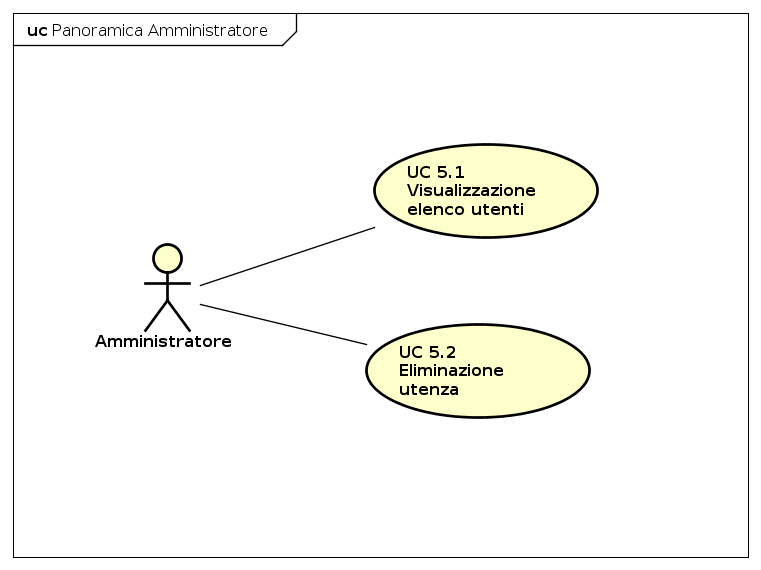
\includegraphics[width=17cm, height= 20cm]{img/PanoramicaAmministratore.png} 
\caption{Panoramica Amministratore}
\end{figure}


\subsubsection{UC 5.1 - Visualizzazione dashboard}

\begin{itemize}
\item \textbf{Attore}: Amministratore; 
\item \textbf{Descrizione}: L'amministratore accede alla propria dashboard personale e può effettuare modifiche al sistema;
\item \textbf{Precondizione}: L'amministratore si è autenticato;
\item \textbf{Postcondizione}: L'amministratore è all'interno della sua dashboard.
\end{itemize}

\subsubsection{UC 5.2 - Visualizzazione utenti registrati}

\begin{itemize}
\item \textbf{Attore}: Amministratore;
\item \textbf{Descrizione}: L'amministratore visualizza l'elenco degli utenti registrati nel sistema;
\item \textbf{Precondizione}: L'amministratore si trova nella dashboard;
\item \textbf{Postcondizione}: L'amministratore visualizza tutti gli utenti registrati nel sistema.
\end{itemize}

\subsubsection{UC 5.3 - Filtraggio utenti}
\begin{itemize}
\item \textbf{Attore}: Amministratore;
\item \textbf{Descrizione}: L'amministratore ha la possibilità di ricercare gli utenti a partire dal loro nome o dalla loro tipologia di utenza;
\item \textbf{Precondizione}: L'amministratore visualizza la lista di utenti registrati;
\item \textbf{Postcondizione}: L'amministratore visualizza la lista degli utenti in base ai filtri applicati.
\end{itemize}

\subsubsection{UC 5.4 - Visualizzazione dettaglio utente}
\begin{itemize}
\item \textbf{Attore}: Amministratore;
\item \textbf{Descrizione}: L'amministratore visualizza in dettaglio un utente specifico;
\item \textbf{Precondizione}: L'amministratore visualizza la lista degli utenti;
\item \textbf{Postcondizione}: L'amministratore visualizza le informazioni personali dell'utente.
\end{itemize}


\subsubsection{UC 5.5 - Eliminazione utenza}
\begin{itemize}
\item \textbf{Attore}: Amministratore;
\item \textbf{Descrizione}: L'amministratore elimina un'utenza dal sistema;
\item \textbf{Precondizione}: L'amministratore visualizza l'elenco degli utenti registrati nel sistema;
\item \textbf{Postcondizione}: L'amministratore ha eliminato l'utenza dal sistema;
\item \textbf{Flusso degli eventi}: L'amministratore seleziona l'utenza e procede all'eliminazione.
\end{itemize}


\subsubsection{UC 5.6 - Visualizzazione richieste sviluppatori}
\begin{itemize}
\item \textbf{Attore}: Amministratore;
\item \textbf{Descrizione}: L'amministratore visualizza tutte le richieste degli utenti che vogliono ottenere il ruolo di sviluppatore nel sistema;
\item \textbf{Precondizione}: L'amministratore si trova nella dashboard;
\item \textbf{Postcondizione}: L'amministratore visualizza l'elenco delle richieste in sospeso.
\end{itemize}

\subsubsection{UC 5.7 - Attivazione utenza sviluppatore}
\begin{itemize}
\item \textbf{Attore}: Amministratore;
\item \textbf{Descrizione}: L'amministratore attiva un utente che ha fatto richiesta come sviluppatore;
\item \textbf{Precondizione}: L'amministratore visualizza la lista delle richieste in sospeso degli sviluppatori;
\item \textbf{Postcondizione}: L'utenza dello sviluppatore è stata attivata e lo sviluppatore può quindi accedere al sistema;
\item \textbf{Flusso degli eventi}:  L'amministratore seleziona la richiesta dell'utente e la attiva, permettendogli di autenticarsi nel sistema.
\end{itemize}

\subsubsection{UC 5.8 - Rifiuto richiesta sviluppatore}
\begin{itemize}
\item \textbf{Attore}: Amministratore;
\item \textbf{Descrizione}: L'amministratore rifiuta la richiesta avanzata da uno sviluppatore;
\item \textbf{Precondizione}: L'amministratore visualizza la lista delle richieste in sospeso degli sviluppatori;
\item \textbf{Postcondizione}: L'utenza dello sviluppatore è stata rifiutata;
\item \textbf{Flusso degli eventi}: L'amministratore seleziona la richiesta dell'utente e la rifiuta.
\end{itemize}


